% Created 2021-01-19 Tue 09:50
% Intended LaTeX compiler: pdflatex
\documentclass[11pt]{article}
\usepackage[utf8]{inputenc}
\usepackage[T1]{fontenc}
\usepackage{graphicx}
\usepackage{grffile}
\usepackage{longtable}
\usepackage{wrapfig}
\usepackage{rotating}
\usepackage[normalem]{ulem}
\usepackage{amsmath}
\usepackage{textcomp}
\usepackage{amssymb}
\usepackage{capt-of}
\usepackage{hyperref}
\usepackage{minted}
\author{Adam Prügel-Bennett}
\date{\today}
\title{Git Instructions}
\hypersetup{
 pdfauthor={Adam Prügel-Bennett},
 pdftitle={Git Instructions},
 pdfkeywords={},
 pdfsubject={},
 pdfcreator={Emacs 26.3 (Org mode 9.1.9)}, 
 pdflang={English}}
\begin{document}

\maketitle
\tableofcontents


\section{Overview}
\label{sec:orgedaaa25}
\href{https://git-scm.com/book/en/v2/Getting-Started-About-Version-Control}{Pro Git Web}
\begin{center}
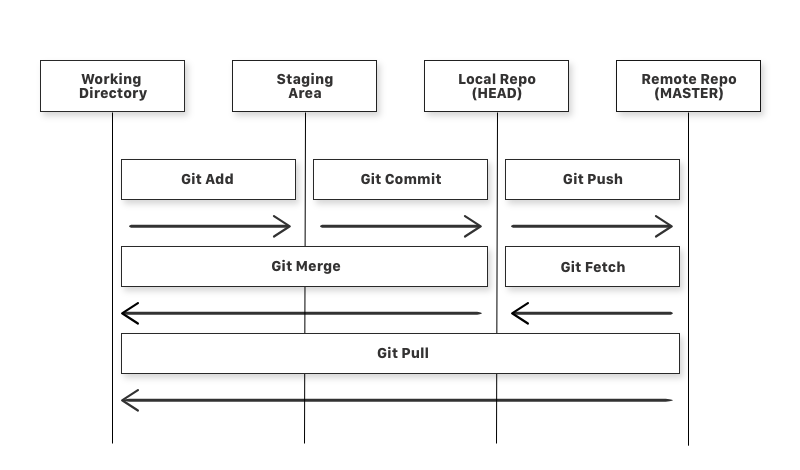
\includegraphics[width=.9\linewidth]{./git.png}
\end{center}

\section{Staging}
\label{sec:orgf2368b2}
\begin{itemize}
\item git add [file]
\item git add .
\end{itemize}

\section{Local Repo (Head)}
\label{sec:orge5d9e42}
\begin{itemize}
\item git commit -m 'message'
\end{itemize}

\subsection{Submitting to Github (master)}
\label{sec:orgd92bd12}
\begin{itemize}
\item \url{https://github.com/adamP-B/nopLearning}
\begin{itemize}
\item git push -u main master
\end{itemize}
\end{itemize}

\subsection{Branching}
\label{sec:orgc7f9a89}
\begin{itemize}
\item git branch newBranchName
\begin{itemize}
\item create a new branch (doesn't do anything)
\end{itemize}
\item git chechout branchName
\begin{itemize}
\item switching to new branch (set HEAD to branch)
\end{itemize}
\item git merge anotherBranchName
\item git log --oneline --decorate --graph --all
\begin{itemize}
\item look at branches
\end{itemize}
\end{itemize}

\section{Useful info}
\label{sec:org5ebf23f}
\begin{itemize}
\item git status
\item git log
\end{itemize}

\section{GPU Server}
\label{sec:org4349bb1}
\begin{itemize}
\item ssh athenadirect
\item Don’t forget to set the env variable CUDA\(_{\text{VISIBLE}}\)\(_{\text{DEVICES}}\)=x where
x is the gpu id (0..3 or a set 0,1,4) \& nvidia-smi
\end{itemize}
\end{document}
